\chapter{Implementacija}

\section{Osnovni koncepi}

U projektu se koriste model klase koje prate JavaBeans specifkaciju. Zastupljena je i upotreba osnovnih Java kolekcija, klasičnih nizova i kolekcije ArrayList(). Također, korištene su mape kako bi se primijenilo stečeno znanje (između ostalog da se izlistaju sve Aviokompanije, koje imaju Avion prijavljen avion u bazi). 

\section{Baza podataka}

Za bazu podataka je korištena SQLite baza podataka. Organizirana je kao standardna relaciona baza podataka čiji je Entity-Relationship-Diagram (ERD) dat na sljedećoj slici:
\begin{figure}[h]
	\centering
	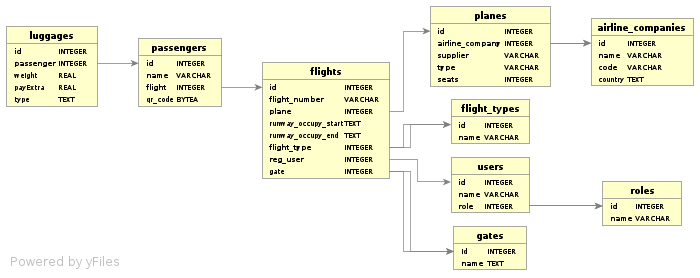
\includegraphics[width=0.9\linewidth]{Slike/ERD}
	\caption{ERD baze podataka}
	\label{fig:erd}
\end{figure}

Treba napomenuti da je baza dizajnirana u DB Browser for SQLite alatu, dok je ERD generisan u DB Visualizer alatu.


\section{Koncepti objektno orjentiranog programiranja}

Koncepti OOP-a (nasljeđivanje, polimorfizam i enkapsulacija) iskorišteni su pri kreiranju ove aplikacije. Najviše su korišteni za implementaciju različitih vrsta prtljaga. Osnovna, apstraktna klasa jeste AbstractLuggage, iz koje su izvedeni prvo Luggage, a zatim i Hand Luggage, te Additional Luggage. Kompletan dijagram klasa nije dio ovog izvještaja, zbog veličine, ali se nalazi u prilogu. Dijagram klasa je generisan korištenjem alata Umbrello.

\section{Grafički interfejs}

Prilikom implementiranja grafičkog interfejsa korišteni su razni GUI elementi. Funkcije koje se nalaze unutar tih elemenata su validirane unutar kontrolera unutar kojih se nalaze listeneri, koji osiguravaju validan unos podataka. Korišteno bidirekcionalno povezivanje polja. Implementirana je i opcija search unutar Airlines, koji vrši pretraju aviokompanija po nazivu. Za tu svrhu su korišteni streamovi, te je ta opcija implemetirana unutar glavnog kontrolera.

Uzeti su u obzir koncepti dobrog dizajna korisničkog interfejsa (Gestalt principi) gdje su svi logički vezani elementi grupisani i na ekranu. 
Za prikaz validnih/nevalidnih polja pozivamo se na .css file, te se postavlja određena boja u zavisnosti od toga da li je polje validno ili ne. Također, podešeno je da prozori ne mogu biti Resizable.

\section{Datoteke}

Datoteke su korištene pri generisanju QR koda, korištenjem biblioteke ZXing. Korišteno je zapisivanje u datoteku qrcode.png (klasa Utills), koja se poslije koristi za generisanje Boarding Pass izvještaja.

\section{Enumi}

Enumi se koriste u izvedenoj klasi Additional Luggage, za odabir između različitih tipova dodatne prtljage. Definirana su tri različita tipa: Metal, Clothes, Money.

\section{Interface}

U projektu se koristi jedan interfejs FlightInterface, u kojem su definirane dvije metoda, te kasnije implementirane u Flights, te pozvane u Mainu. Prva metoda obavještava da je preostalo još sat vremena do boardinga, dok druga obavještava da je "posljednji voz" za ukrcavanje, te se javlja 30 minuta prije leta (obje su vezane za metodu startOfUsingTheRunway). Obavješenje se šalje kao ispis u konzolu. Ovo se može poslije reimplementirati da šalje i na drugačiji način (recimo na eksterni displej ili kiosk). Za sada je samo kao \textit{proof of concept}.

\section{Generika}

Iako nisu korištene generičke klase i metode u striktnom smislu, korištena je evaluacija tipova objekata koji predstavljaju prtljagu, na osnovu unešenih parametara. Obzirom da u startu nisam razmišljala o korištenju ovih koncepata, naknadni dizajn bi zahtjevao jako mnogo pomjena unutar kompletnog projekta.

\section{Mrežno programiranje i tredovi}

Mrežno programiranje se koristi da bi se sa Countries REST API-a (\url{https://restcountries.eu/rest/v2/all}) dobavila lista zemalja. Ovo je riješeno u okviru klase AirlineController koja popunjava ComboBox za odabir zemlje. Ujedno je iskorišten thread kojim se ovo dobavljanje i parsiranje JSON objekta izvršava u pozadini. Korisnik je u okviru UI-a obaviješten, korištenjem ProgressIndicator klase iz JavaFX-a da je u toku dobavljanje (\textit{loading}).

\section{Lokalizacija / Internacionalizacija}

Lokalizacija / Internacionalizacija je zastupljena u dijelu View, gdje korisnik može odabrati između različitih jezika: bosanski, engleski, španjolski, njemački, francuski, ruski, arapski i kineski jezik.

\section{Funkcionalno programiranje}

Funckionalno programiranje je iskorišteno na više mjesta, korištenjem lambda funkcija. Npr. u slučaju listenera u kontrolerima ili kao event handling prilikom dobavljanja odgovora iz REST servisa.

\section{Izvještaji}

Unutar projekta postoje tri različita izvještaja koji se mogu kreirati: Flights Report, Passengers Report, Users Report. Sva tri izvještaja se formiraju na principu formiranja Java kolekcije, koja se zatim prosljeđuje Jasper kompajleru. Na taj način se formira izgled izvještaja, koji se kasnije prikazuje na ekranu.

\section{Maven}

Korišten je Maven alat za automatsku izgradju koda. Uvedene su sljedeće dependencies: sqlite-jdbc, jasperreports, zxing (biblioteka za rad sa QR kodovima), tornado (biblioteka za DateTimePicker komponentu). Pored toga, za testiranje su korišteni junit5 i testfx biblioteke. Svi dependecies se mogu pogledati detaljno u pom.xml datoteci. Svim ovim smo postigli i da se generiše izvršni .jar file u target folderu (rpr-projekat-1.0-SNAPSHOT-jar-with-dependencies.jar) koji se može pokrenuti i iz komandne linije.

\section{Testiranje}

Za testiranje ovoga projekta korišteni su JUnit testovi, kroz Junit5 i TestFX biblioteke. Ukupno je generisano 250 testova, pri čemu je Code Coverage po klasama 88\%, dok je pokrivenost metoda 80 \%. U nastavku je dato objašnjenje zbog čega nije potpuna automatska pokrivenost koda.\\

Željela bih naglasiti da se znalo dešavati da MainTest klasa testova (u kojoj se nalaze TestFX testovi), ponekad padne i prije nego se pokrene, kao i da neki testovi znaju pasti kada se pokrenu svi TestFX testovi uz Code Coverage (pojedinačno prolaze svi, bez Code Coverage). Pokušala sam dati problem riješiti tako da stavljam pauze pomoću funkcije Thread.sleep(), međutim, i dalje se zna desiti da neki padnu pri pokretanju svih. Ostatak testiranja koji nedostaje do 100\%, za koji nisam našla pogodan način kako automatski testirati, jesu Reports (Users, Passengers, Flights), te Lokalizacija. 

\section{Vlastiti izuzeci}

Vlastiti izuzeci su iskorišteni u dijelu koda gdje se unosi broj sjedišta unutar aviona.

\section{Pokretanje}

Najjednostavnije pokretanje je direktno iz IntelliJ IDE-a. Da bi se to omogućilo, potrebno je u postavkama Mavena u dijelu Runner označiti polje (CheckBox) \textit{Delegate IDE build/run actions to Maven}. Nakon toga, potrebno je desnim klikom na klasnu Main.java odabrati Run i IDE će pozvati Maven build sekvencu, te pokrenuti aplikaciju.


